\chapter{Introduction to Fluid-Structure Interaction}
The interaction between fluids and structures can be observed all around us in nature.
From a flag waving in the wind to a large windmill at sea, when we breath in air and our lungs expand, when our hearts fill up with blood and muscles contract to push blood into our arteries, are all examples of fluids and structures interacting. A flag waving in the wind is mainly air(fluid) exerting force on the flag(structure), making the flag flutter. However, the structure can also move the fluid. 
When we breathe air into our lungs, our diaphram contracts and moves downward, increasing the space in our chest cavity making the lungs expand. As the lungs expand air is sucked through the mouth and nose, filling up the lungs. In this manner both fluid and structures can exert force, and consequently interact with each other. 

A bridge is a rigid structure interacting with wind(fluid), this interaction is an example of Fluid-Structure Interaction(FSI).
A profound example of wind interacting with a bridge, is the collapse of the Tacoma Narrows Bridge in 1940 \cite{Billah1991}. The bridge collapsed only two months after being opened. The collapse was due to strong winds(64 km/h) interacting with the structure, making the bridge flutter and ultimately collapse. No human lives were lost in the collapse, but a Cocker Spaniel named Tubby left behind in a car was not that lucky and lost its life in the bridge collapse. \newline

\begin{figure}
\centering
\begin{minipage}{.51\textwidth}
  \centering
  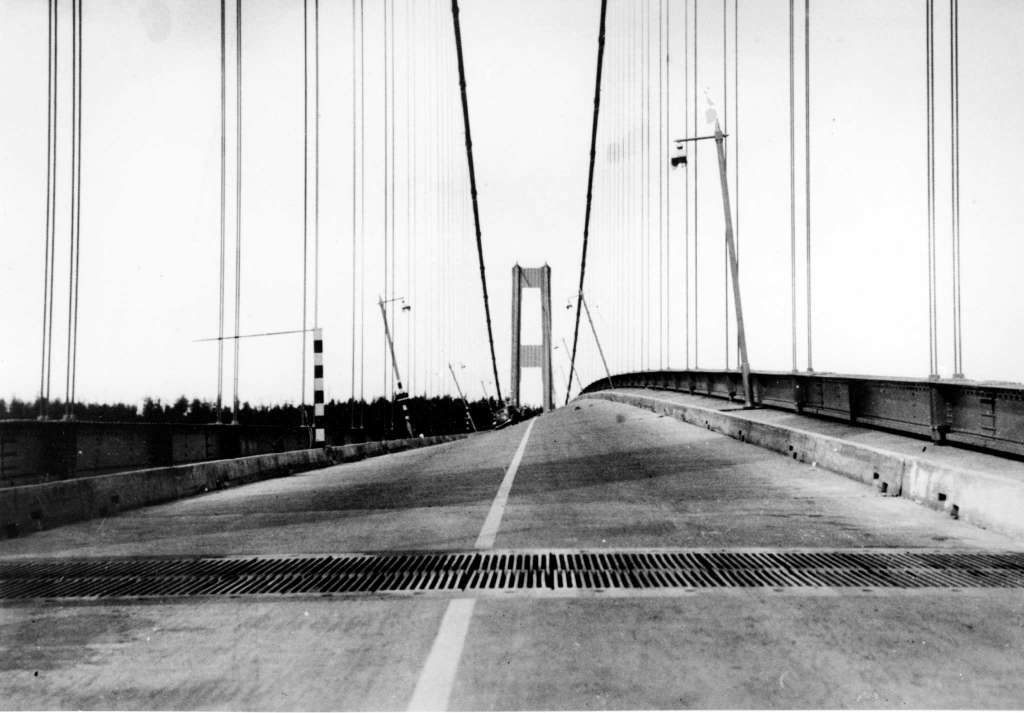
\includegraphics[width=.95\linewidth]{./IntroductionToFSI/tacoma2.jpeg}
  \caption{Tacoma Narrows bridge still standing with large deformations}
  \label{fig:test1}
\end{minipage}%
\begin{minipage}{.50\textwidth}
  \centering
  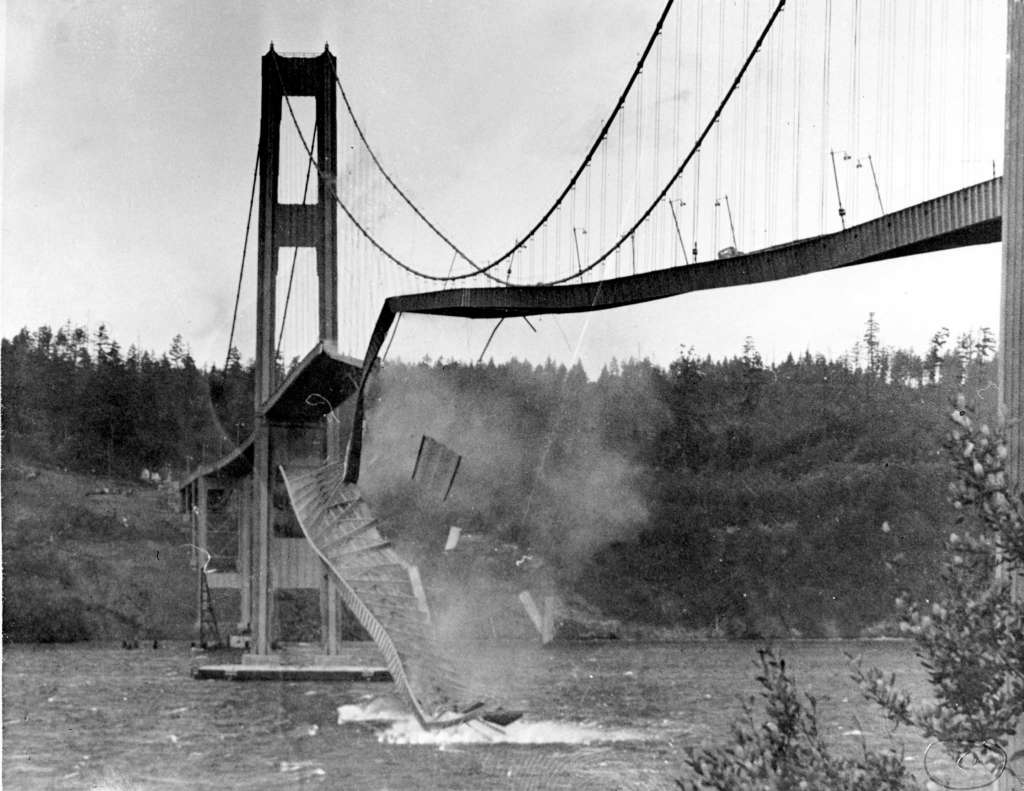
\includegraphics[width=.95\linewidth]{./IntroductionToFSI/tacoma3.jpeg}
  \caption{Tacoma Narrows bridge collapsed}
  \label{fig:test2}
\end{minipage}
\end{figure}

Modeling FSI is used today when constructing for instance windmills. Windmills are normally considered stiff relative to the flowing air, hence giving a big difference in density between fluid and structure. The structure will in the case of a windmill only give rise to small deformations. However, modeling FSI in hemodynamics(dynamics of blood flow) deems more challenging. In the latter cases the densities in fluid and structure are more similar and blood flow usually induces large deformations in the veins and arteries. In both cases the fluid flow tends to transitions towards turbulence. All of these cases have challenges which gives the need to have rigid stabile FSI solvers. \newline

A branch of fluid dynamics is called Computational Fluid Dynamics, where computers and numerical analyses are used to solve fluid problems.
I would argue that a similar name is used for FSI, namely \textit{Computational Fluid Structure Interaction} (CFSI). However in the literature FSI is used to describe CFSI and the name FSI will be used in this thesis. Also, even though FSI is Fluid-\textit{Structure} Interaction, the word solid will also be used to describe a structure. \newline

The main goal of this master thesis is to build a framework to solve FSI problems, investigating different approaches and schemes. The framework will be validated and verified using the \textit{Method of Manufactured Solutions}, accompanying a classic, well known benchmark, known to test the robustness of a FSI solver.



\begin{comment}
Fluid-Structure Interaction problem can be observed all around us in nature, from large industrial engineering complexes to the smallest blood vessels in the human body. A large scale example is the collapse of the Tacoma Narrows Bridge that collapsed in 1940 only two months after being opened. The collapse was due to aero-elastic fluttering from strong winds. No human life was lost in the collapse, but a cocker spaniel name Tubby left in a car was not so lucky. The construction of windmills are a second example of the Fluid-Structure Interaction problem. Todays windmills are rigid and hence giving a big difference in density between fluid and structure, $ \rho_s >> \rho_f $. The structure will therefore only give rise to small deformations. However applying FSI to hemodynamics( dynamics of blood flow ) deems more challenging. One FSI hemodynamic problem are inter-cranial aneurysms, which are balloon shaped geometries often occurring where a blood vessel splits into two parts, due to weak vessel walls. Bursting of one of these aneurysms in the skull can have fatale consequences. With fluid and structure densities more equal than the previous example, the structure has an elastic character giving under the right circumstances large deformations. The blood flow also transitions to turbulent flow. This combination gives the need for a rigid stabile solver. Therefore the main goal of this master thesis is to build a framework to solve the FSI problem, investigating different approaches and schemes. The framework will be validated and verified using MMS, companying a wide range of benchmarks.  
\end{comment}

